\documentclass[areasetadvanced]{scrartcl}

\usepackage[utf8]{inputenc}
\usepackage[T2A]{fontenc}
\usepackage[english,russian]{babel}

\usepackage[footskip=1cm,left=25mm, right=15mm, top=20mm, bottom=20mm]{geometry}
\usepackage{setspace}
\usepackage{amsmath, amssymb}  % Объединено в одну строку
\usepackage{graphicx}
\usepackage{tikz}
\usetikzlibrary{arrows.meta}
\usepackage{float}
\usepackage{dashrule}
\usepackage{fancyhdr} % оформление отчёта
\usepackage{hyperref} % оформление отчёта
\usepackage{parskip}
\usepackage{textcomp, enumitem}
\usepackage{indentfirst}
\usepackage{graphicx}
\usepackage{algorithm}
\usepackage{algpseudocode}
\usepackage{array}  % Для использования команды m{}
\usepackage{geometry}
\usepackage{afterpage}
\usepackage{minted}
\setcounter{secnumdepth}{3}  % Включает нумерацию для subsubsection
\setcounter{tocdepth}{3}     % Включает subsubsection в содержание
\usepackage{listings} % Если используете listings

\tikzstyle{block} = [rectangle, rounded corners, minimum width=3cm, minimum height=1cm, text centered, draw=black, fill=lightgray]

\setkomafont{sectioning}{\normalfont\bfseries} % для заголовков разделов и подразделов
\setkomafont{section}{\normalfont\Large\bfseries}
\setkomafont{subsection}{\normalfont\large\bfseries}
\setkomafont{subsubsection}{\normalfont\large\bfseries}
\setkomafont{paragraph}{\normalfont\large\bfseries} % для заголовков параграфов (если они есть)

\lstset{
  language=Haskell,
  basicstyle=\ttfamily\small,
  keywordstyle=\color{blue}\bfseries,
  stringstyle=\color{red},
  commentstyle=\color{green!70!black},
  numbers=left,
  numberstyle=\tiny,
  stepnumber=1,
  numbersep=10pt,
  showstringspaces=false,
  breaklines=true,
  frame=single
}

\setcounter{tocdepth}{2}
\begin{document}
	\thispagestyle{empty}
	\begin{center}
		\large{МИНОБРНАУКИ РОССИИ} \par
		\vspace{0.3cm}
		\normalsize
		{ФЕДЕРАЛЬНОЕ ГОСУДАРСТВЕННОЕ АВТОНОМНОЕ ОБРАЗОВАТЕЛЬНОЕ УЧРЕЖДЕНИЕ ВЫСШЕГО ОБРАЗОВАНИЯ} \par
		\vspace{0.3cm}
		\textbf{\guillemotleft САНКТ-ПЕТЕРБУРГСКИЙ ПОЛИТЕХНИЧЕСКИЙ}
		\textbf{УНИВЕРСИТЕТ ПЕТРА ВЕЛИКОГО\guillemotright} \par
		\vspace{0.3cm}
		{Институт компьютерных наук и кибербезопасности}\par
		{Высшая школа технологий искусственного интеллекта}\par
	\end{center}
	\vfill
	\begin{center}
		{\large Отчёт по дисциплине \guillemotleft Математическая логика\guillemotright}\par
		{\huge   Лабораторная работа №1 
		
		\guillemotleft Лексический анализатор\guillemotright}\par
            {\huge Вариант \textbf{№14}}
         
	\end{center}
	\vfill
	\begin{flushleft}
		Студент: \hspace{1.8cm} \rule[0pt]{2.5cm}{0.5pt}\hfill Салимли Айзек Мухтар Оглы\par
		\vspace{1.5cm}
		Преподаватель: \hspace{0.55cm} \rule[0pt]{2.5cm}{0.5pt}\hfill  Востров Алексей Владимирович
	\end{flushleft}
	\vspace{0.5cm}
	\begin{flushright}
		\guillemotleft \rule[0pt]{0.8cm}{0.5pt}\guillemotright \rule[0pt]{2cm}{0.5pt} 20\rule[0pt]{0.5cm}{0.5pt} г.
	\end{flushright}
	\vfill
	\begin{center}
		Санкт-Петербург, 2025
	\end{center}
	\newpage
	\tableofcontents
	\newpage
\section*{Введение}
	\addcontentsline{toc}{section}{Введение}

    В отчете описана реализация web приложения лексического анализатора.
    Цель задачи состоит в реализации лексического анализатора, который будет проводить лексический анализ входного текста в соответствии с заданным вариантом. Программа пораждает таблицу лексем с указанием их типов и значений.
    Реализация была дополнена иными ключевыми словами, операторами и функторами. 
\begin{sloppypar}
    Был собран stack проект, код программы написан на языке Haskell2010, с конфигурацией Cabal 3.0.0, GHC 9.12.2 в интегрированной среде разработки visual studio code.
    Использованные библиотеки: 
\end{sloppypar}
\begin{itemize}
    \item base >= 4.14.0.1 \&\& < 5 --стандартная библиотека
    \item threepenny-GUI --библиотека для создания веб интерфейса
    \item data.char --библиотека для работы с символами
\end{itemize}
    \textbf{Указанный вариант - №14.} \\
    Правила:
    \begin{itemize}
        \item Входной текст содержит операторы цикла while \dots do и do \dots while
        \item Разделитель символом $;$
        \item Операторы условия содержат знаки сравнения $=$, $>$, $<$
        \item Вещественные числа
        \item Знак присваевания $:=$
        \item Вещественные числа могут начинатся с точки$*$
    \end{itemize}
    Дополнения:
    \begin{itemize}
        \item Монады
        \item Тип-данных Monad
        \item Тип-данных String
        \item Функторы: <>, $<\$>$,$.$, map, fmap
        \item Стрелка Клейсли: $>>=$
        \item Лямбда-функции: \textbackslash n
        \item Семантика циклов: while \dots do и do \dots while
    \end{itemize}
    Не компелируемые лексемы:
    \begin{itemize}
        \item Комментарии типа: $--$
        \item Комментарии типа: $//$
        \item Комментарии типа: $/* */$
    \end{itemize}

\newpage
\section{Постановка задачи}

Написать программу, которая выполняет лексический анализ входного текста в
соответствии с заданием и порождает таблицу лексем с указанием их типов и значений.
\begin{enumerate}
    \item Подготовить несколько вариантов программы в виде текста на входном языке.
    \item Программа должна выдавать сообщения о наличие во входном тексте ошибок, которые могут быть обнаружены на этапе лексического анализа.
    \item Длина идентификатора и строковых констант ограничена 16 символами, только латиница. 
    \item Программа должна допускать наличие комментариев неограниченной длины во входном файле. 
    \item Построить синтаксические диаграммы.
\end{enumerate}
\newpage

\section{Математическое описание}

\subsection{Математическая модель программы}

Лексический анализатор принимает на вход строку символов \( w \) и выдает последовательность токенов \( T = (t_1, t_2, \dots , t_n) \).

\[
F_{\text{lexer}} : \Sigma^* \rightarrow T^*
\]

, где:
\begin{itemize}
    \item \( \Sigma^* \) - множество всех возможных строк над алфавитом \( \Sigma \);
    \item \( T^* \) - множество всех возможных последовательностей токенов;
    \item \( t_i \in T \) - токены.
\end{itemize}

Лексический анализатор строится на основе регулярных языков и грамматик Хомского.

\subsection{Грамматика Хомского}

Формальная грамматика Хомского — это набор \( G = (N, \Sigma, P, S) \), состоящий из:
\begin{itemize}
    \item \( N \) - конечного множества нетерминалов;
    \item \( \Sigma \) - конечного множества терминальных символов (алфавит);
    \item \( P \) - множества продукций (правил);
    \item \( S \in N \) - начального символа.
\end{itemize}

\subsection{Типы грамматик Хомского}

Существует четыре типа грамматик Хомского, но в контексте\\ лексического анализа рассматриваются два:

\textbf{Тип 3 (Регулярные грамматики)}:
\[
A \rightarrow \alpha B \quad \text{или} \quad A \rightarrow \alpha
\]
, где \( A, B \) — нетерминалы, а \( \alpha \) — терминал.

\textbf{Тип 2 (Контекстно-свободные грамматики)}:
\[
A \rightarrow \gamma, \quad \text{где } A \text{ - нетерминал, } \gamma \text{ - последовательность терминалов и нетерминалов.}
\]

Тип 1 (КЗ грамматики):
\[
\alpha A \beta \rightarrow \alpha \gamma \beta
\]
где \( A \) — нетерминал, \( \alpha, \gamma, \beta \) — строки из \( (N \cup \Sigma)^* \), и \( |\gamma| \geq |\beta| \).

\newpage
\subsection{Диаграммы}

На рисунке 1, представлена синтаксическая диаграмма последующей программы.

    \begin{figure}[h]
        \centering
        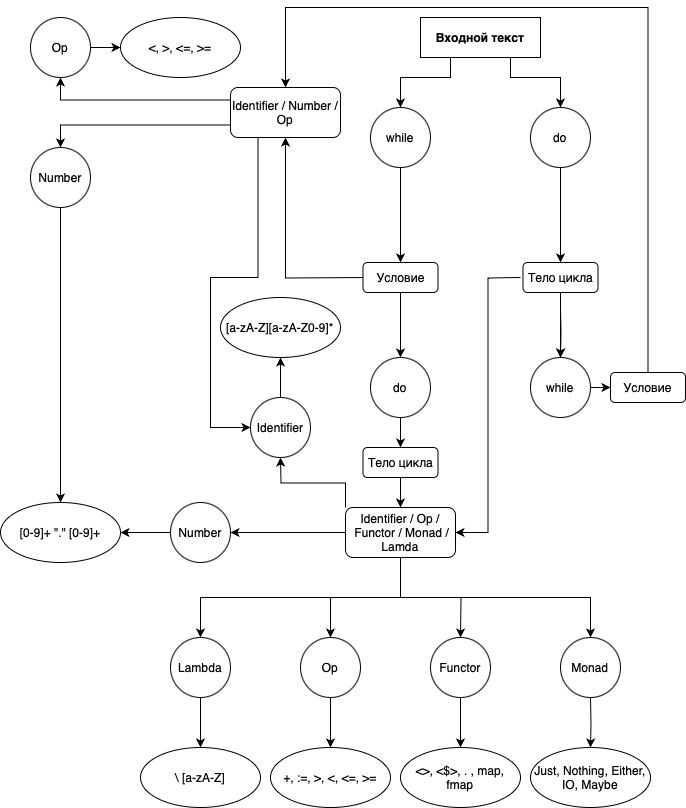
\includegraphics[width=0.6\textwidth]{СинтДиагр.drawio.png}
        \caption{Синтаксическая диаграмма.}
        \label{fig:syntdiag}
    \end{figure}

На рисунке 2, представлена лексическая диаграмма:
\begin{figure}[H]
        \centering
        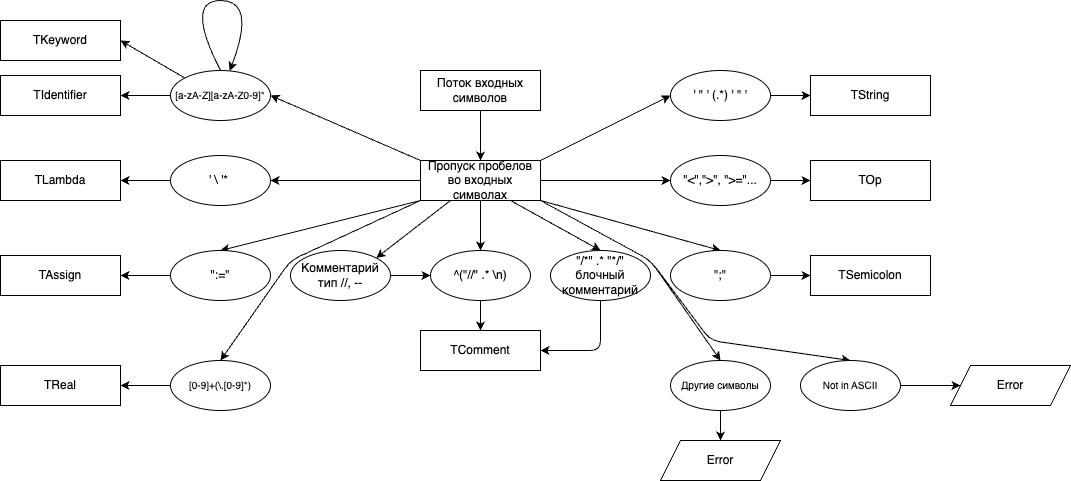
\includegraphics[width=0.7\textwidth]{LexDiagram.png}
        \caption{Лексическая диаграмма.}
        \label{fig:syntdiag}
\end{figure}

\newpage

\section{Программная реализация}
\subsection{Реализация}

Программа была разделена в проекте \textbf{stack} на управляющую логику (\textbf{Lib.hs}) и веб-интерфейс (\textbf{Main.hs}). В качестве веб-интерфейса была выбрана библиотека \textbf{threepenny-gui} из Hackage.

\subsection{Lib.hs}
\textbf{Определение токенов (типов лексем):}
\begin{lstlisting}
data Token
    = TWhile
    | TDo
    | TKeyword String
    | TIdentifier String
    | TReal Double
    | TAssign
    | TOp String
    | TSemicolon
    | TString String
    | TComment String
    | TLambda String
    deriving (Show, Eq)
\end{lstlisting}

Функция \textbf{tokenLexeme :: Token -> String} преобразует токен в строку:
\begin{lstlisting}
tokenLexeme :: Token -> String
tokenLexeme t = case t of
  TWhile        -> "while"
  TDo           -> "do"
  TKeyword s    -> s
  TIdentifier s -> s
  TReal d       -> show d
  TAssign       -> ":="
  TOp op        -> op
  TSemicolon    -> ";"
  TString s     -> s
  TComment s    -> s
  TLambda s     -> s
\end{lstlisting}

Функция \textbf{lexer} разбирает строку на токены и ошибки, вызывая \textbf{lexInternal}:
\begin{lstlisting}
lexer :: String -> ([Token], [String])
lexer input =
    let (ts, es) = lexInternal input
    in if not (null es)
        then (ts, es)
        else
          let e2 = checkNonLatinForNonComment ts
          in (ts, e2)
\end{lstlisting}

Функция \textbf{lexInternal} рекурсивно разбивает строку на токены:
\begin{lstlisting}
lexInternal :: String -> ([Token],[String])
lexInternal [] = ([], [])
lexInternal (c:cs)
    | isSpace c = lexInternal cs
    | c=='/' && take 1 cs == "/" = ...
    | c=='-' && take 1 cs == "-" = ...
    | isAlpha c = lexIdentOrKeyword (c:cs)
    | isDigit c || c=='.' = lexNumber (c:cs)
    | otherwise =
        let (toks, errs) = lexInternal cs
        in ([], ("Unexpected character: " ++ [c]) : errs)
\end{lstlisting}

Функция \textbf{executeProgram} выполняет разбор программы и имитацию циклов:
\begin{lstlisting}
executeProgram :: String -> Either String String
executeProgram s =
    let (ts, es) = lexer s
    in if not (null es)
        then Left (unlines es)
        else
          let noComm = filter (not . isComment) ts
          in case noComm of
              [ TWhile, TIdentifier i1, TOp "<", TReal lim, TDo, TSemicolon
              , TIdentifier i2, TAssign, TIdentifier i3, TOp "+", TReal st
              , TSemicolon]
                  | i1==i2 && i2==i3 -> execWhileLoop 0 lim st 0

              [ TDo, TIdentifier i1, TAssign, TIdentifier i2, TOp "+", TReal st
              , TSemicolon, TWhile, TIdentifier i3, TOp "<", TReal lim, TSemicolon]
                  | i1==i2 && i2==i3 -> execDoWhileLoop 0 lim st 0

              _ -> Left "Unsupported program format"
\end{lstlisting}
\newpage
\subsection{Main.hs}

Содержит UI-функции библиотеки \textbf{Threepenny-GUI}.
Функция \textbf{setup :: Window -> UI()} настраивает интерфейс:
\begin{lstlisting}
setup window = do
  return window # set title "Haskell UI"
  on UI.click recognizeButton $ \_ -> do
    txt <- get value inputBox
    if all isSpace txt
      then element outputDiv # set text "Enter text or press \"Generate\""
      else do
        let (tokens, errors) = lexer txt
        if not (null errors)
          then element outputDiv # set text ("Errors:\n" ++ unlines errors)
          else do
            let assigns = buildAssignMap tokens
            let (comments, nonComments) = separateComments tokens
            let (rows, _) = foldl
                              (\(acc,counter) tk ->
                                  let (row3, newC) = tokenToRow assigns tk counter
                                  in (acc ++ [row3], newC))
                              ([], 1)
                              nonComments

            tableMain <- buildMainTable rows
            tableComm <- buildCommentTable comments
            element outputDiv # set children [tableMain, tableComm]
\end{lstlisting}

Для предотвращения зацикливания была создана функция сброса:
\begin{lstlisting}
on UI.click resetButton $ \_ -> do
  element inputBox  # set value ""
  element outputDiv # set text "Reset"
\end{lstlisting}
\newpage 
\section{Результаты программы}
На рисунках 2 - 13 представлены результаты выполнения лексического анализатора. 

\subsection{Варианты}
\begin{figure}[H]
    \centering
    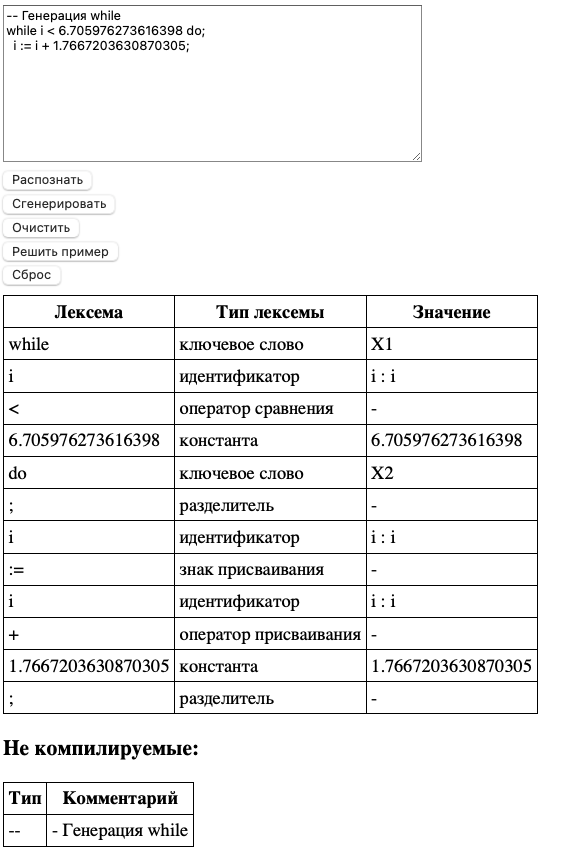
\includegraphics[width=0.7\textwidth]{Original.png}
    \caption{Стандартный вариант}
    \label{fig:syntdiag}
\end{figure}

\begin{figure}[H]
    \centering
    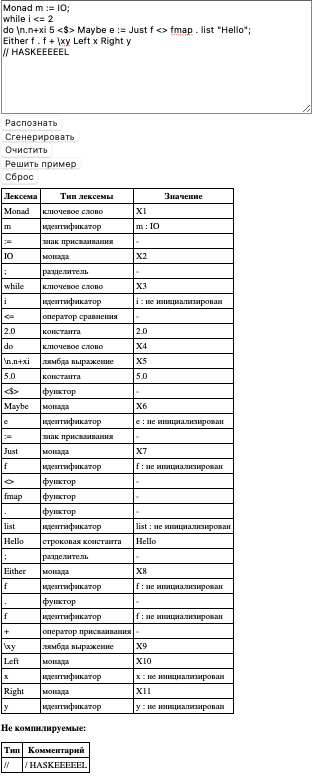
\includegraphics[width=0.5\textwidth]{Large.png}
    \caption{Расширенный вариант}
    \label{fig:syntdiag}
\end{figure}

\subsection{Исключения и ошибки анализа}

\begin{figure}[H]
    \centering
    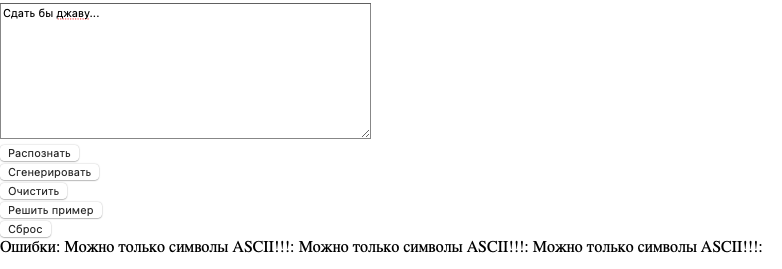
\includegraphics[width=0.7\textwidth]{OnlyASCII.png}
    \caption{Ошибка ввода кириллицы}
    \label{fig:syntdiag}
\end{figure}

\begin{figure}[H]
    \centering
    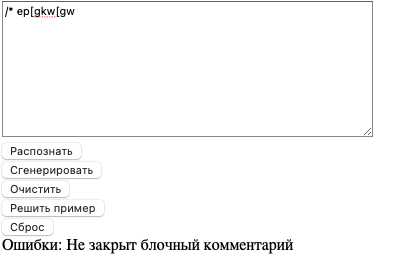
\includegraphics[width=0.7\textwidth]{ErrorComment.png}
    \caption{Ошибка: не закрыт блочный комментарий}
    \label{fig:syntdiag}
\end{figure}

\begin{figure}[H]
    \centering
    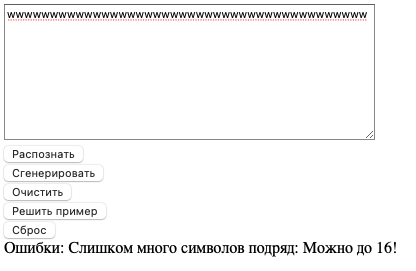
\includegraphics[width=0.7\textwidth]{More16.png}
    \caption{Ошибка: длина лексемы больше 16}
    \label{fig:syntdiag}
\end{figure}

\begin{figure}[H]
    \centering
    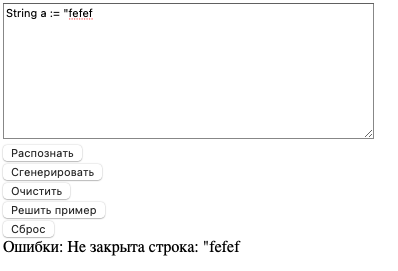
\includegraphics[width=0.7\textwidth]{StringError.png}
    \caption{Ошибка: не закрыта строка}
    \label{fig:syntdiag}
\end{figure}

\begin{figure}[H]
    \centering
    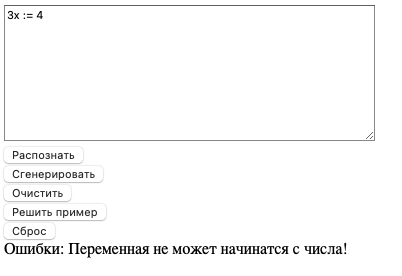
\includegraphics[width=0.7\textwidth]{ErrorNotN.png}
    \caption{Ошибка: неверное начало индентификатора}
    \label{fig:syntdiag}
\end{figure}

\begin{figure}[H]
    \centering
    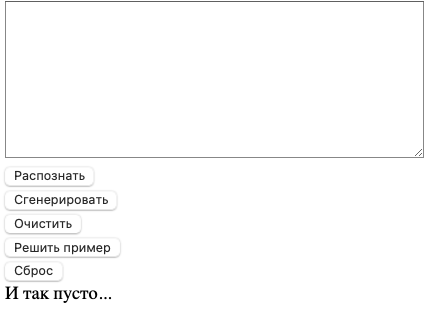
\includegraphics[width=0.7\textwidth]{Empty.png}
    \caption{Ошибка: попытка очистить пустое окно}
    \label{fig:syntdiag}
\end{figure}

\begin{figure}[H]
    \centering
    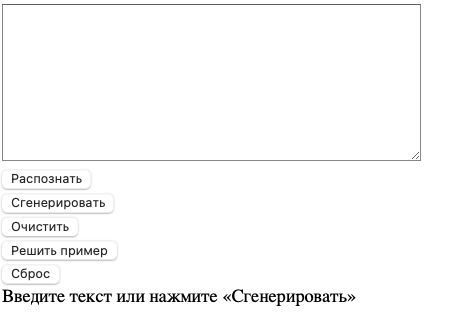
\includegraphics[width=0.7\textwidth]{FullEmpty.png}
    \caption{Ошибка: респознать пустое окно}
    \label{fig:syntdiag}
\end{figure}

\begin{figure}[H]
    \centering
    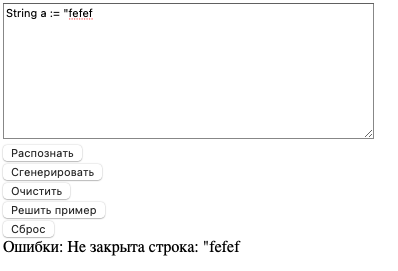
\includegraphics[width=0.7\textwidth]{StringError.png}
    \caption{Ошибка: не закрыта строка}
    \label{fig:syntdiag}
\end{figure}

\subsection{Особые случаи}
\begin{figure}[H]
    \centering
    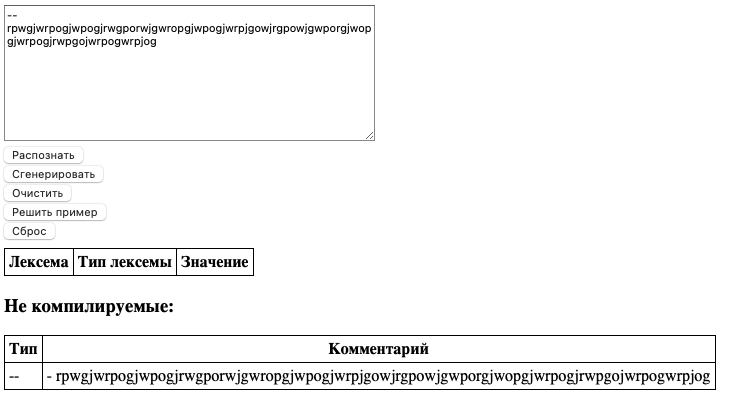
\includegraphics[width=0.7\textwidth]{LargeComment.png}
    \caption{Разрешен большой комментарий}
    \label{fig:syntdiag}
\end{figure}

\subsection{Семантика}
\begin{figure}[H]
    \centering
    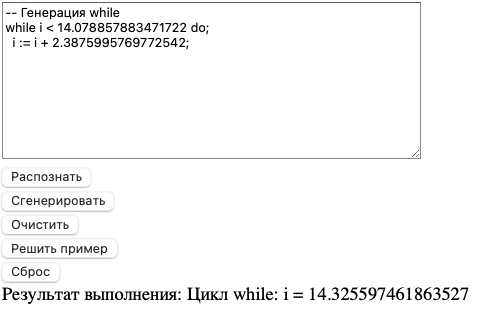
\includegraphics[width=0.7\textwidth]{WhileSem.png}
    \caption{Семантика цикла}
    \label{fig:syntdiag}
\end{figure}

\subsection{Выбор текстового файла}
\begin{figure}[H]
    \centering
    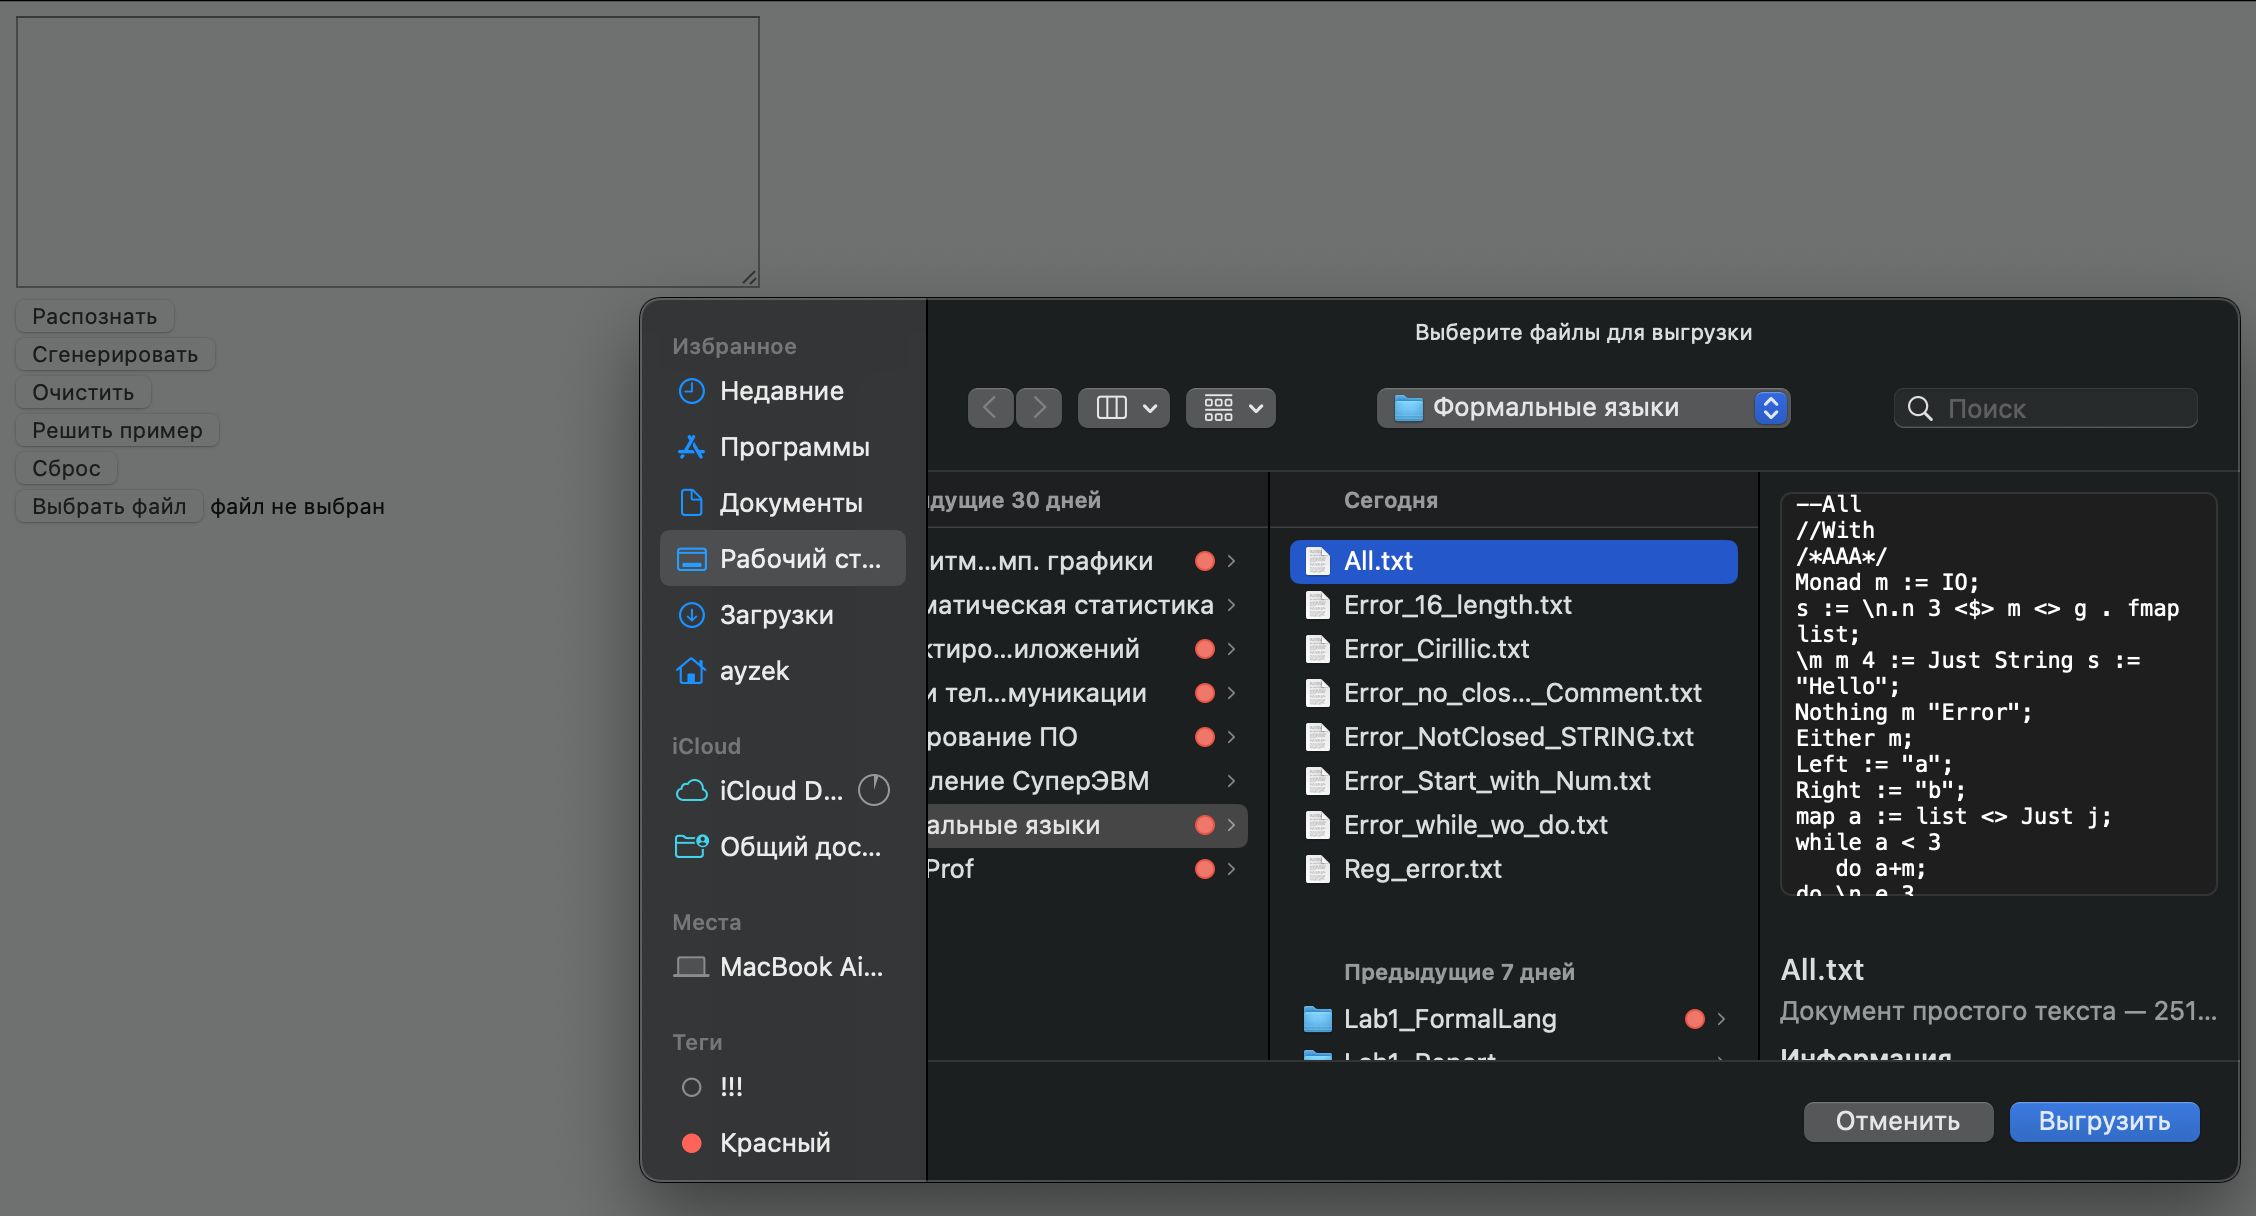
\includegraphics[width=0.7\textwidth]{FileOpen.png}
    \caption{Выбор текстового файла}
    \label{fig:syntdiag}
\end{figure}
Преведены все случаи ошибок и вариантов работы программы.
\newpage

\section*{Заключение}
\addcontentsline{toc}{section}{Заключение}
\begin{sloppypar}
В результате выполнения лабораторной работы №1, был реализован синтаксический (лексический) \\анализатор, распознающий ключевые слова, вещественные числа, идентификаторы, операторы, функторы, разделители и строки.
Лексический анализатор, основан на логике грамматик Хомского, с подстановкой токенов как терминалов и нетерминалов.
Так же приведина синтаксическая диаграмма программы. Так же были разработаны дополнения расширяющие грамматику.
\end{sloppypar}
\textbf{Дополнения к грамматике}:
\begin{enumerate}
    \item Ключевые слова
    \subitem Monad, String
    \item Монады
    \subitem Just, Either, Nothing, Maybe, Left, right
    \item Функторы
    \subitem fmap, map, ., \_, <>, <\$>
    \item Строки
    \subitem '"'(.*)'"'
    \item Другие типы комментариев
    \subitem /* */, --
\end{enumerate}
\textbf{Дополнения к синтаксису}:
\begin{enumerate}
    \item do не может быть без while
    \item while не может быть без do
    \item Monad, String - ключевые слова-типы после которых идет идентификатор
\end{enumerate}
\textbf{Дополнения к семантике}:
\begin{enumerate}
    \item Семантика цикла do \dots while
    \item Семантика цикла while \dots do
\end{enumerate}
\textbf{Плюсы}: 
\begin{enumerate}
    \item Лексеры написаны чистыми функциями
    \item Использование паттерн-матчингов
    \item Haskell, идеально подходит для задач написания парсинга, компиляторов и т.д 
    \subitem Ленивые списки и ленивые функции подходят для легкой работы написания парсинга
    \subitem Все ошибки типов выявляются на этапе компиляции
    \subitem С pattern-matching Haskell легко строить синтаксические деревья
\end{enumerate}
\textbf{Минусы}: 
\begin{enumerate}
    \item При некоторых компбинациях семантика цикла может вызвать бесконечную рекурсию
    \item Нет автоматического позиционирования 
    \item Не проверяется последовательность 
    \item Для использованных библиотек, необходима версия GHC >= 9.11.0
\end{enumerate}
\textbf{Масштабируемость}:
\begin{enumerate}
    \item Отслежевание позиций
    \item Выделение типов токенов из библиотеки Threepenny-GUI
    \item Дополнение до лексического автомата
\end{enumerate}
\newpage
\section*{Список литературы}
\addcontentsline{toc}{section}{Список литературы}
\begin{enumerate}
    \item \begin{sloppypar}Востров, А. В. Математическая логика [Электронный ресурс]. Режим доступа: https://tema.spbstu.ru/compiler/ (последний визит: 18.03.2025). \end{sloppypar}
    \item Сети, Р.; Ахо, А. Компиляторы: принципы, технологии и инструменты / Р. Сети, А. Ахо. – М.: Издательство «Наука», 2006. – С. 104.
\end{enumerate}
\end{document}